% !TeX spellcheck = es_ES
%%%%%%%%%%%%%%%%%%%%%%%%%%%%%%%%%%%%%%%%%
% Stylish Article
% LaTeX Template
% Version 2.1 (1/10/15)
%
% This template has been downloaded from:
% http://www.LaTeXTemplates.com
%
% Original author:
% Mathias Legrand (legrand.mathias@gmail.com) 
% With extensive modifications by:
% Vel (vel@latextemplates.com)
% Final ACS by:
% Juan Barbosa
% License:
% CC BY-NC-SA 3.0 (http://creativecommons.org/licenses/by-nc-sa/3.0/)
%
%%%%%%%%%%%%%%%%%%%%%%%%%%%%%%%%%%%%%%%%%
\documentclass[fleqn,11pt]{SelfArx}
%\usepackage[superscript]{cite}
\usepackage{wrapfig}
\usepackage{rotating}
\usepackage{subcaption}
\usepackage[numbers]{natbib}
%----------------------------------------------------------------------------------------
%	ARTICLE INFORMATION
%----------------------------------------------------------------------------------------

\JournalInfo{Fisicoqu\'imica avanzada, No. 2, 23/11/2018} % Journal information
\Archive{ }

\PaperTitle{Isoterma de adsorci\'on SBA-15} %
%\Keywords{Keyword1 --- Keyword2 --- Keyword3} % Keywords - if you don't want any simply remove all the text between the curly brackets
%\newcommand{\keywordname}{Keywords} % Defines the keywords heading name

%----------------------------------------------------------------------------------------
%	ABSTRACT
%----------------------------------------------------------------------------------------

\Abstract{
	El presente documento contiene una breve introducci\'on a los materiales mesoporosos, sus formas de s\'intesis y las t\'ecnicas de caracerizaci\'on. Adem\'as, se menciona la s\'intesis de Zhao para la obtenci\'on de SBA-15. A partir de esto se analizan los pasos claves de la preparaci\'on, y se obtienen par\'ametros BET para los datos de una isoterma, los cuales corresponden con: $v_m = 154\pm 1$ STP y $c = 500 \pm 200$. Finalmente, se determina el \'area superficial total en $670\pm 4$ m$^2$.
}

%----------------------------------------------------------------------------------------

\begin{document}
	\flushbottom % Makes all text pages the same height
	
	\maketitle % Print the title and abstract box
	
	%\tableofcontents % Print the contents section
	
	\thispagestyle{empty} % Removes page numbering from the first page
	\renewcommand{\tablename}{Tabla} 
	
	
	%----------------------------------------------------------------------------------------
	%	ARTICLE CONTENTS
	%----------------------------------------------------------------------------------------
	
	\section*{Introducci\'on}
	
	Los materiales mesoporosos son aquellos que presentan poros con tama\~nos entre los 20 \r{A} y 500 \r{A} \cite{macnaught_wilkinson_1997}, los mismos han sido ampliamente estudiados por su demanda en reacciones y separaciones de compuestos de alto peso molecular \cite{zhao_1998}. Los materiales mesoporosos se obtienen a partir de variedad de compuestos, siendo los m\'as comunes aquellos de s\'ilica y al\'umina \cite{mitra_bhaumik_paul_2008}. Existen adem\'as algunos ejemplos de \'oxidos de metales de transici\'on como el niobio, t\'antalo, tit\'anio, y zirconio \cite{mitra_bhaumik_paul_2008, lee_lu_kondo_domen_2002,noda_lee_domen_kondo_2008, parvulescu_bonnemann_parvulescu_endruschat_rufinska_lehmann_tesche_poncelet_2001}. En particular, las s\'ilicas porosas presentan propiedades importantes como resistencia mec\'anica, \'area superficial y tama\~no del poro uniforme. Los mayores exponentes de los compuestos mesoporosos basados en el silicio son el MCM-41, sintetizado en 1992 por Mobil Corporation con una geometr\'ia unidimensional cil\'indrica \cite{zhao_1998}. Por otro lado la SBA-15 (\textit{tipo de material Amorfo Santa Barbara} del ingl\'es \textit{Santa Barbara Amorphous type material}), sintetizada en 1997 en la Universidad de California en Santa Barbara, es un tipo de material mesoporoso con poros de tama\~nos entre 46 y 300 \r{A} y geometr\'ia bidimencional hexonal \cite{zhao_1998}.
	
	Debido a la escala de las nanopart\'iculas, se han desarrollado una gran variedad de condiciones para explorar el direccionamiento estructural que presentan las interacciones electroest\'aticas, puentes de hidr\'ogeno y van der Waals, en la s\'intesis de compuestos mesoporosos \cite{zhao_1998}. En el caso del MCM-41 y la SBA-15, para el primero se hace uso de surfactantes cati\'onicos, mientras que para la segunda se usan no i\'onicos \cite{zhao_1998}. Para la preparaci\'on de la SBA-15 es posible usar gran variedad de tensoactivos, los cuales le agregan diferentes propiedades al s\'olido obtenido. A pesar que un \'unico surfactante es suficiente, los mejores resultados son obtenidos usando una combinaci\'on de dos tensoactivos conocida como Pluronic 123, el cual consiste en una cadena polim\'erica de tres bloques de copol\'imeros (\autoref{eq: pluronic}): \'oxido de polietileno (EO), \'oxido de polipropileno (PO), y nuevamente \'oxido de polietileno (EO). Los surfactantes anteriores hacen parte de una familia de tensoactivos muy usados en la emulsificaci\'on, solubilizaci\'on, lubricaci\'on, adem\'as de ser usados como espumantes y farmace\'uticos \cite{zhao_1998}.
	\begin{equation} \label{eq: pluronic}
	\ce{EO_{20}-PO_{70}-EO_{20}} \qquad \text{Pluronic 123}
	\end{equation}
	
	El procedimiento general para la obtenci\'on de compuestos mesoporosos es la formaci\'on de miscelas, la polimerizaci\'on y crecimiento de la red estructural, y posterior calcinaci\'on con el objetivo de eliminar el surfactante y restos de disolvente en la estructura porosa.	En la s\'intesis de la estructura mesoporosa mostrada en el presente documento se hace uso de tetraetil ortosilicato (TEOS) como fuente de silicio para la formaci\'on de la red estructural, Pluronic 123 como surfactante para la formaci\'on de miscelas, siguiendo la s\'intesis de Zhao \cite{zhao_1998}.
	
	\begin{scheme}[h]
		\centering
		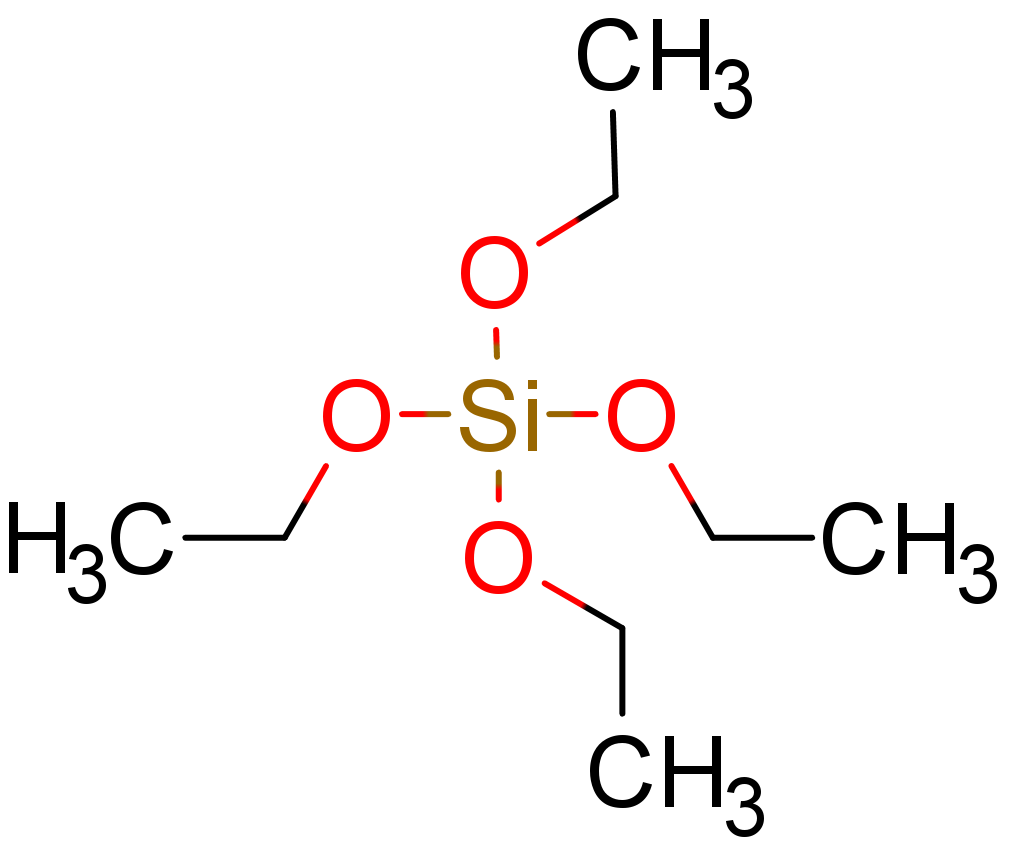
\includegraphics[width=0.4\linewidth]{structures/silicate.png}
		
		\caption{Estructura del tetraetil ortosilicato.}
		\label{scheme: sources}
	\end{scheme}
	
	\begin{scheme*}[ht]
		\centering
		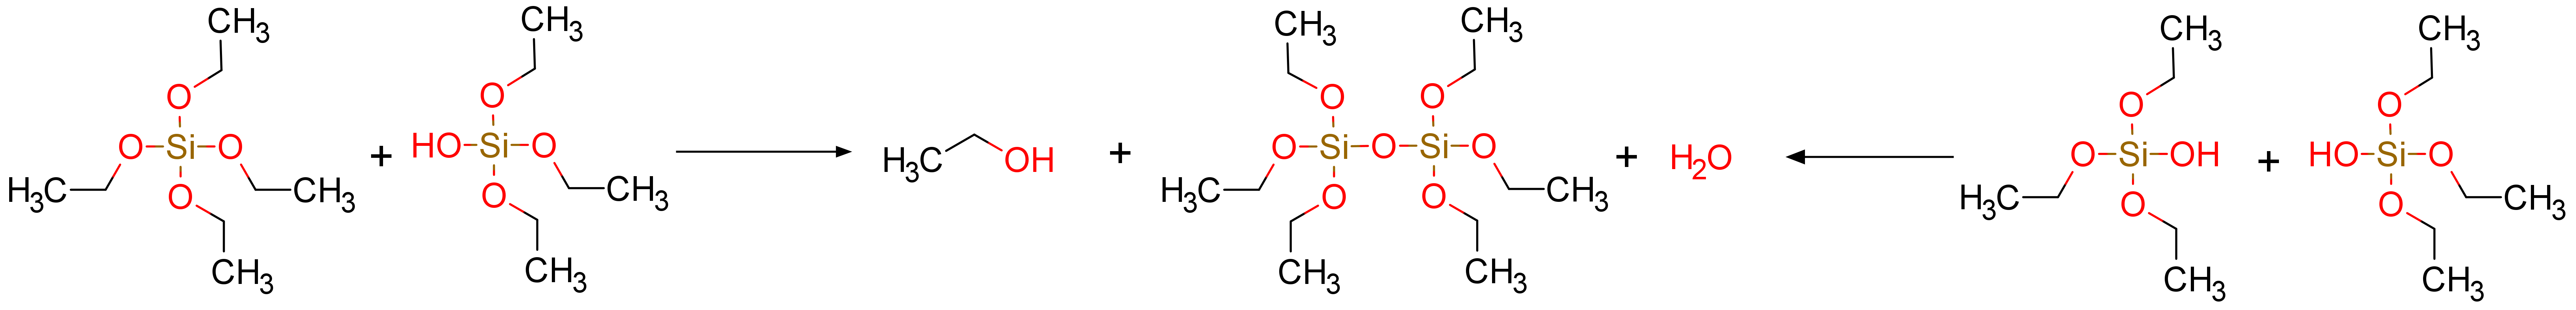
\includegraphics[width=\linewidth]{structures/polysilicate.png}
		\caption{Formaci\'on de una red estructural. De izquierda a derecha la condensaci\'on con salida de etanol, y de derecha a izquierda condensaci\'on de agua.}
		\label{sch: polysilicate}
	\end{scheme*}
	
	La caracterizaci\'on de los compuestos mesoporosos incluye gran variedad de t\'ecnicas, entre las que se encuentran: microsc\'opicas, espectrosc\'opicas, adsortivas, termogravim\'etricas y termodin\'amicas \cite{vargas_legnoverde_giraldo_basaldella_moreno-pirajan_2010}. Las t\'ecnicas de microscop\'ia electr\'onicas son el barrido electr\'onico (SEM) y de transferencia electr\'onica (TEM), la primera se usa con el objetivo de observar la superficie de las nanopart\'iculas y la segunda la estructura interna, que da informaci\'on sobre la porosidad de las mismas. La Fluorescencia de rayos X por energía dispersiva (EDX) permite determinar la relaci\'on silicio-otros elementos en una muestra de SBA-15, y la resonancia magn\'etica nuclear usando el \'angulo m\'agico para el \ce{^{29}Si}, permite obtener informaci\'on sobre los distintos ambientes qu\'imicos del silicio en la muestra \cite{zhao_1998}. La capacidad de adsorci\'on de un material se cuantifica usando isotermas de adsorci\'on. Los termogramas de una muestra permiten conocer la composici\'on de la misma en funci\'on de la temperatura. Finalmente los an\'alisis termodin\'amicos permiten conocer entalp\'ias, y estados qu\'imicos o f\'isicos de la muestra \cite{vargas_legnoverde_giraldo_basaldella_moreno-pirajan_2010}.
	
	Las isot\'ermas de adsorci\'on se realizan con nitr\'ogeno l\'iquido y gaseoso para controlar la temperatura y presi\'on a lo largo del experimento. Para una presi\'on determinada se mide el volumen de nitr\'ogeno obtenido luego de pasar sobre la muestra, dado que se conoce el volumen total introducido es posible calcular el volumen adsorbido por el material. La informaci\'on obtenida se relaciona con la teor\'ia de Brunauer–Emmett–Teller (BET), la cual da cuenta del proceso de adsorci\'on y desorci\'on usando como hip\'otesis: que las mol\'eculas de un gas pueden ser f\'isicamente adsorbidas por una capa de un s\'olido indefinidamente, no existe ninguna interacci\'on entre las capas del s\'olido, y los gases se comportan como gases ideales. La teor\'ia BET permite calcular el \'area superficial de un compuesto mesoporoso. Adem\'as, las curvas de adsorci\'on se encuentran clasificadas por la IUPAC, seg\'un la forma de las mismas. Tipo I cuando solo existe adsorci\'on por monocapa, tipo II cuando se observa una zona plano en la curva an\'aloga a una funci\'on polin\'omica de grado 3, donde la regi\'on en particular se debe a la formaci\'on de la monocapa. Tipo III cuando se observa adsorci\'on por multicapa, y las curvas tipo IV presentan todas las anteriores, en donde el nivel de saturaci\'on se alcanza a una presi\'on menor a la presi\'on de vapor, lo anterior se explica con la condensaci\'on de gas en  regiones capilares de los mesoporos \cite{sing_2001}.
	
	\section{Secci\'on experimental}
	A nivel sint\'etico, la s\'intesis de Zhao consiste en disolver el Pluronic 123 en agua, con la posterior adici\'on de \'acido clorh\'idrico. A la soluci\'on resultante se le adiciona por goteo tetraetil ortosilicato, el s\'olido obtenido se lava con agua en repetidas ocasiones y finalmente es calcinado.
	
	La isoterma obtenida se obtiene usando el equipo Autosorb iQ de Quantachrome Instruments, el cual se encuentra en el grupo de Sólidos Porosos y Calorimetría. Es de resaltar que este instrumento es capaz de medir vol\'umenes de nitr\'ogeno en el rango de presiones relativas ($P/P_0$) de 0.001 a 1.000, adem\'as de incorporar un espectr\'ometro de masas.
	
	Usando una celda especial se cuantifica la masa de la celda, y se adicionan desde 50 a 200 mg de muestra, dependiendo de la porosidad de la misma. Posteriormente tiene lugar la desgasificaci\'on de la muestra, la cual dura cerca de 8 horas, y se usa una rampa de calentamiento que en su punto m\'aximo puede superar los 300 $^\circ$C. Posteriormente se pesa nuevamente la celda con muestra y conociendo la masa de muestra desgasificada se procede a realizar la isoterma de adsorci\'on. Esta consiste en fijar un n\'umero de valores de $P/P_0$, en los cuales se desea tomar una medida de adsorci\'on, para este caso particular se usaron 68 puntos. Usando la cantidad m\'inima de helio el sistema mide el volumen de las tuber\'ias y posteriormente inicia su an\'alisis.	
	
	\section{Resultados y Discusi\'on}
	\begin{figure}[h]
		\centering
		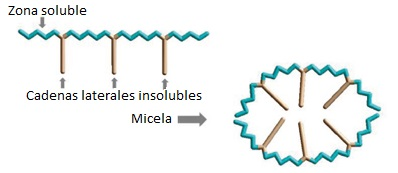
\includegraphics[width=0.8\linewidth]{structures/Micela.jpg}
		\caption{Formaci\'on de micelas por el copol\'imero Pluronic 123. Modificado de \cite{grallert_rangel_yagui_pasqualoto_tavares_2012}.}
		\label{fig: micela}
	\end{figure}
	\pagebreak
	
	 Sobre la s\'intesis se tiene que el Pluronic presenta a sus extremos dos copol\'imeros solubles, mientras que en el medio se encuentra el polipropileno, el cual presenta una cadena lateral poco polar. Los polietilenglicoles de los extremos forman puentes de hidr\'ogeno con el agua, haciendo de los mismos una parte hidrof\'ilica, las cadenas laterales (metilos) del polipropilenglicol forman la parte hidrof\'obica, dando lugar a la formaci\'on de micelas de la forma ilustrada en la \autoref{fig: micela}. Siguiendo con la s\'intesis de Zhao se tiene que el tetraetil ortosilicato en agua, se hidrolisa, y posteriormente puede condensarse con otra mol\'ecula hidrolizada o el \'eter de sililo, dando lugar a la formaci\'on de un enlace silanol como se muestra en el \autoref{sch: polysilicate}, luego de m\'ultiples repeticiones, tiene lugar la formaci\'on de una red alrededor de la estructura cil\'indrica. Una vez adicionada la fuente de silicio, las micelas modifican su geometr\'ia y hebra a hebra se condensa con el \'eter de sililo.
	\begin{scheme}[h]
		\centering
		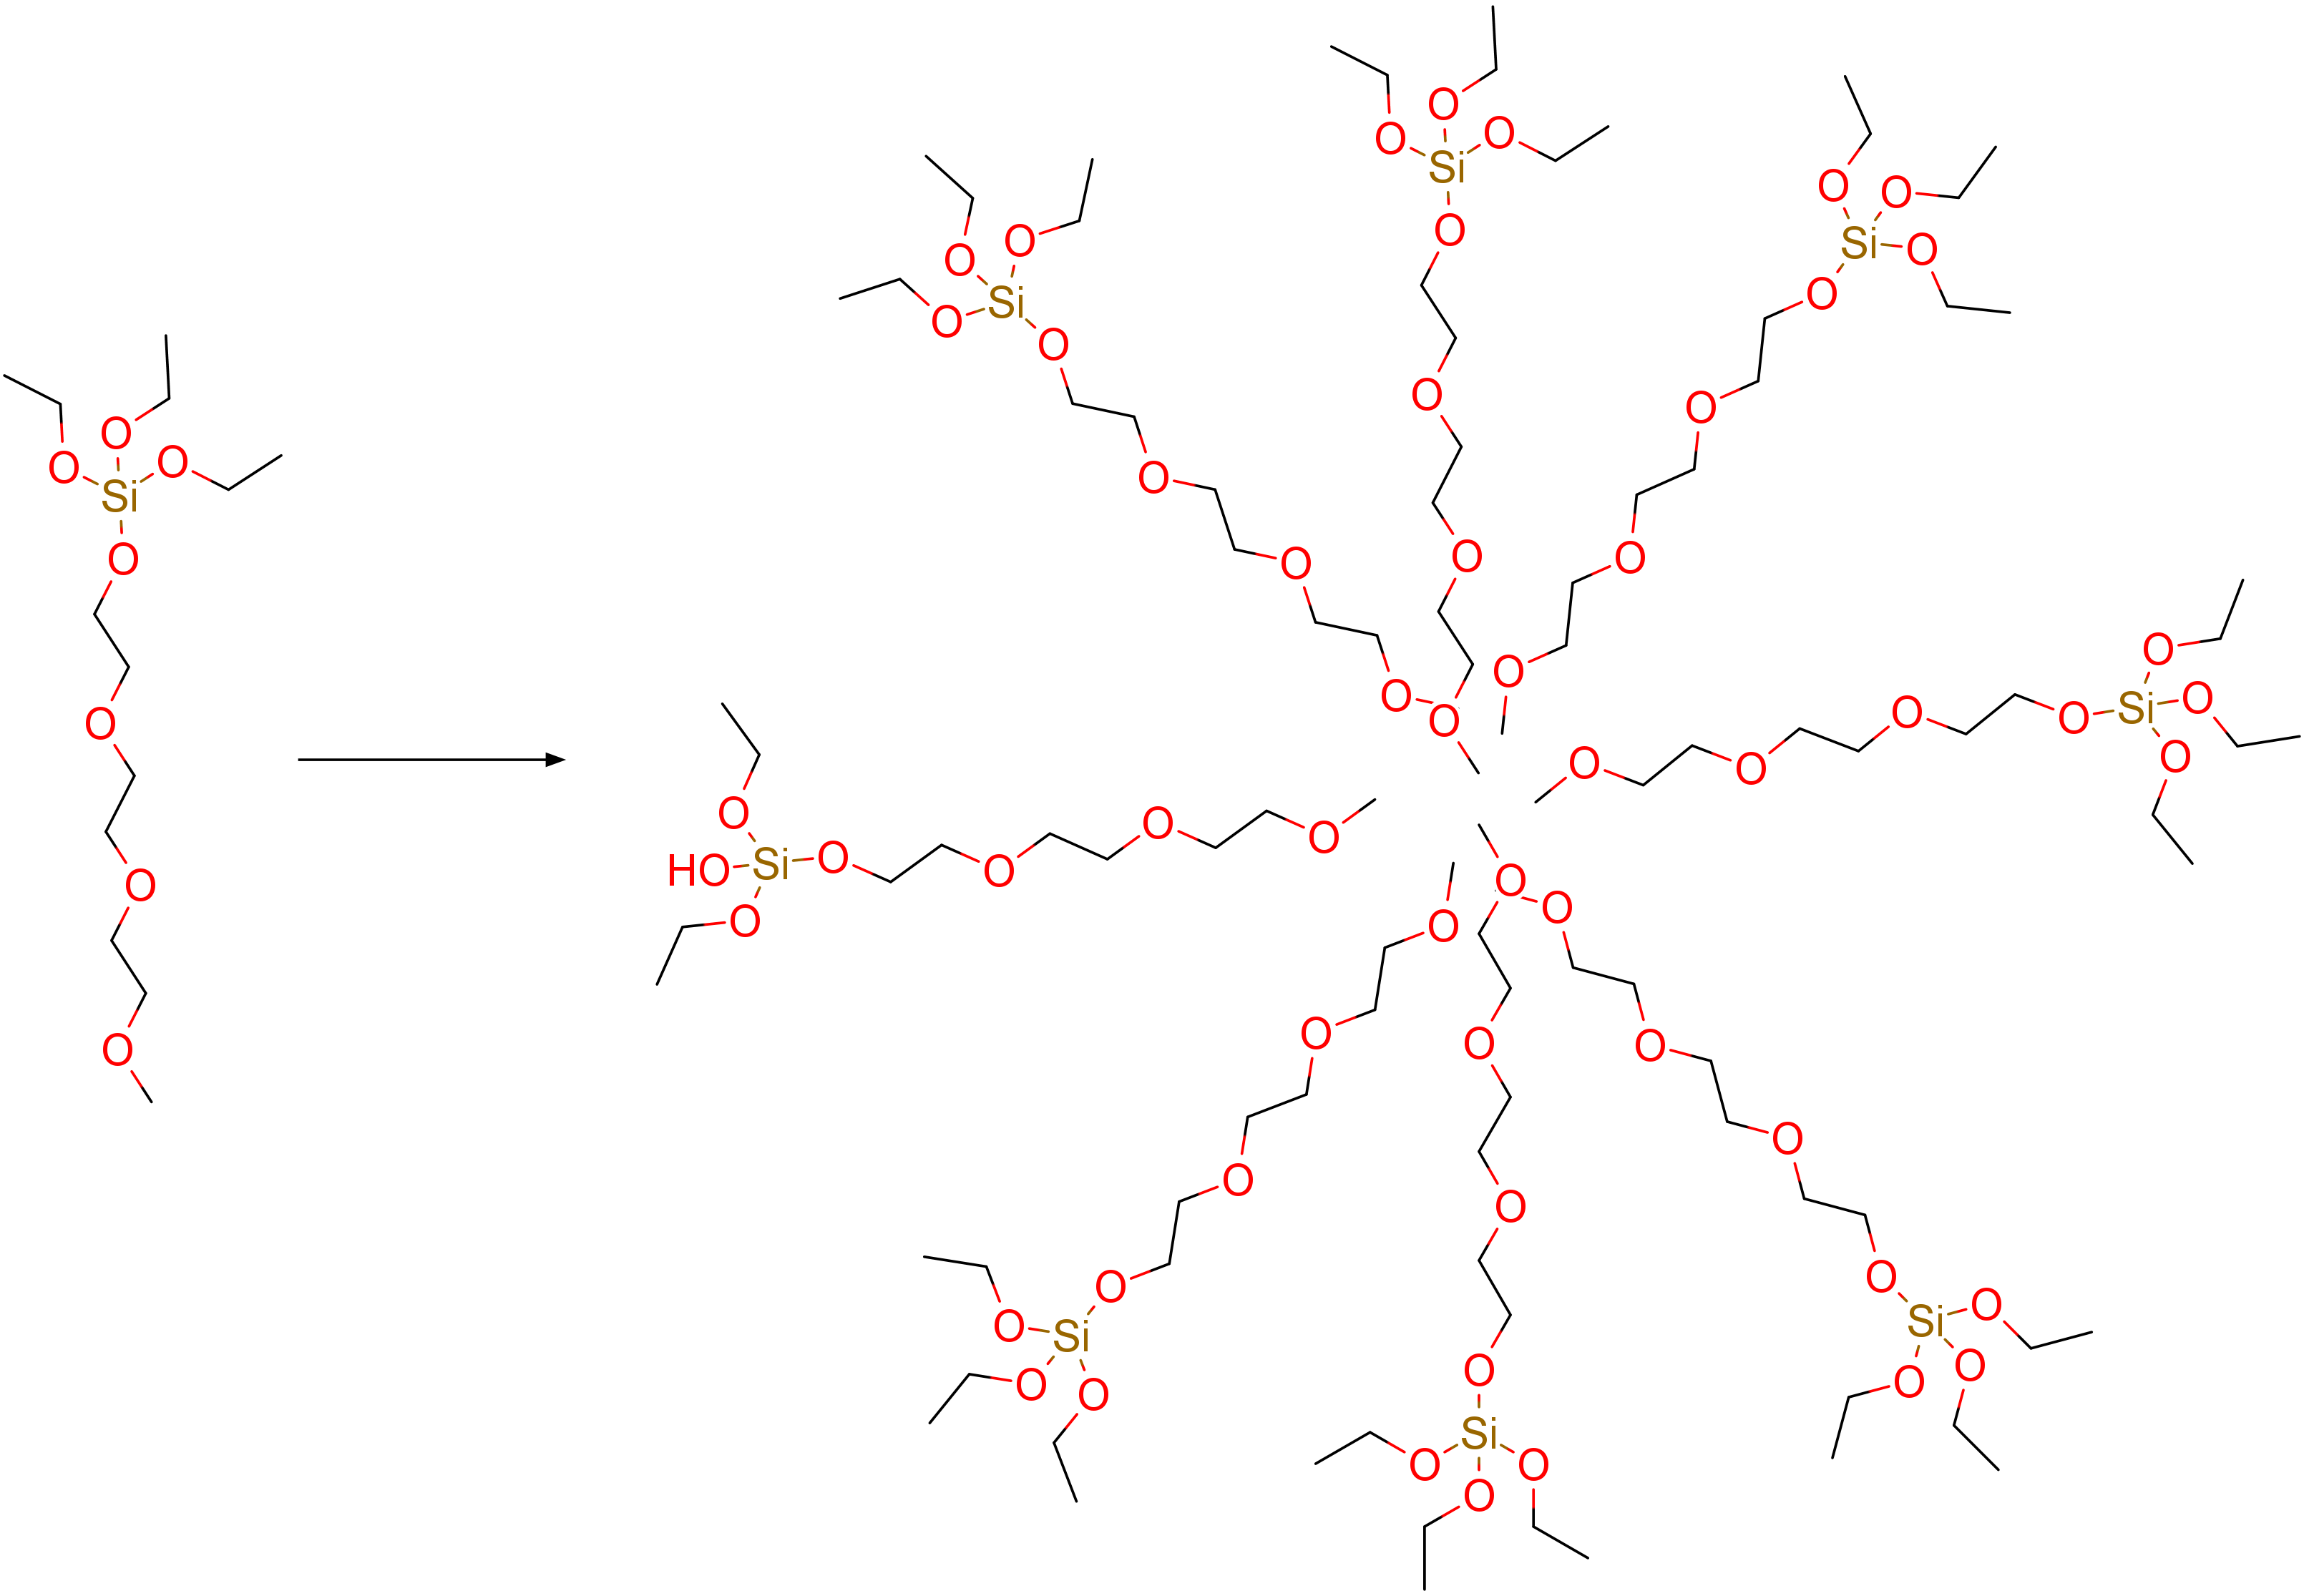
\includegraphics[width=0.95\linewidth]{structures/micelaSi.png}
		\caption{Formaci\'on de las micelas con la incorporaci\'on del silicio \cite{yang_2011}.}
		\label{sch: micelaSi1}
	\end{scheme}
	
	La formaci\'on de micelas en la soluci\'on constituye la primera etapa en la formaci\'on de los compuestos mesoporos. Las hebras se condensan intermolecularmente entre ellas siguiendo lo mostrado en el \autoref{sch: polysilicate}, formando un caparaz\'on de silanol. Con el hidroxilo restante las micelas tienden a unirse formando una estructura tridimensional cil\'indrica como en la \autoref{fig: micela3d}. Incrementando el aislamiento de los grupos m\'as hidrof\'obicos al interior del cil\'indro.
	\begin{figure}[h]
		\centering
		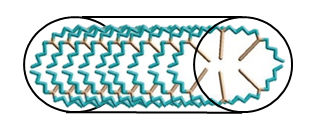
\includegraphics[width=0.8\linewidth]{structures/micela3D.png}
		\caption{Formaci\'on de estructuras cil\'indricas por parte de las micelas.}
		\label{fig: micela3d}
	\end{figure}
	
	Los cilindros se agupan dando lugar a la formaci\'on de estructuras hexagonales. Finalmente, la calcinaci\'on elimina el contenido interno de las estructuras con la descomposici\'on del copolimero que se encuentra en el mismo, obteniendo estructuras mesoporosas.
	
	\begin{figure}[h]
		\centering
		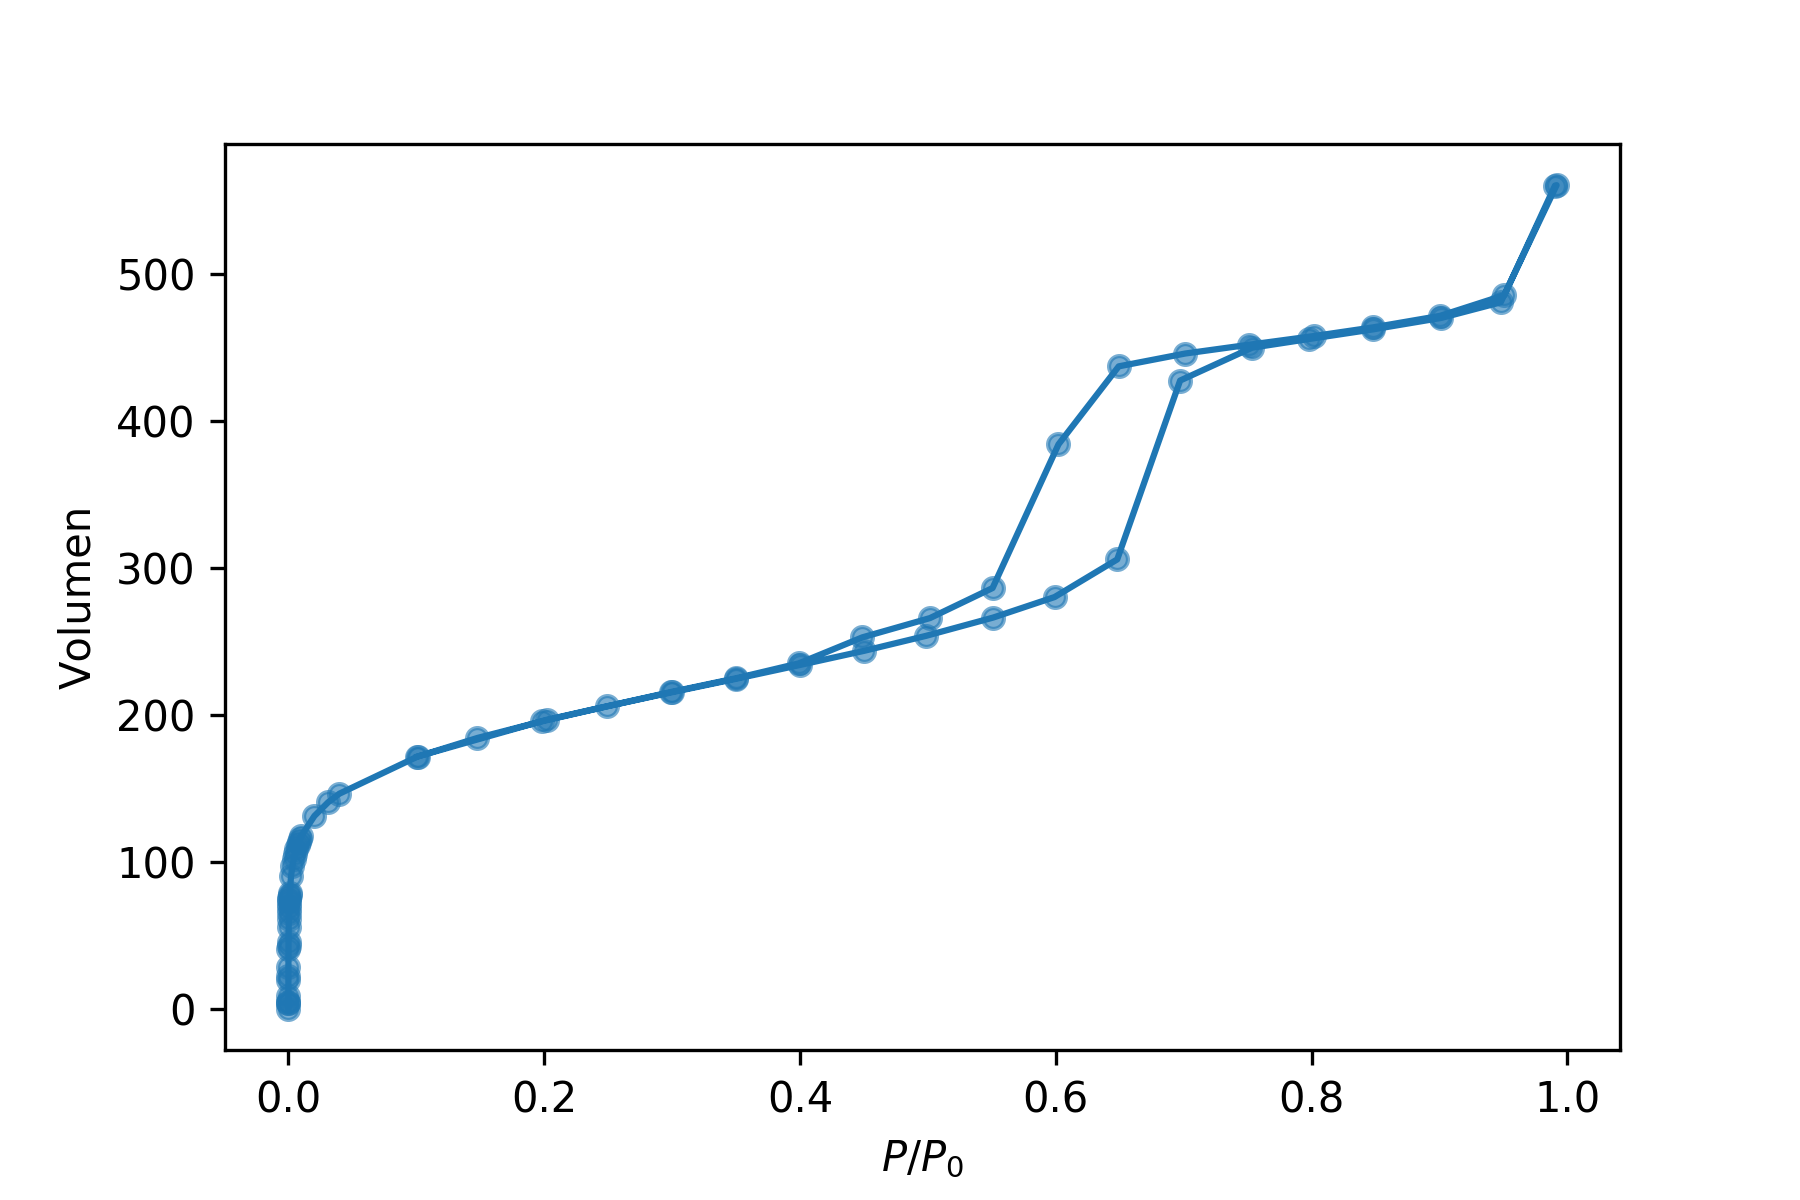
\includegraphics[width=\linewidth]{isoterma}
		\caption{Isoterma de adsorci\'on para la SBA-15. El modelo BET se construye con los siguientes valores: $c = 470$, y $v_m = 154$ cm$^3$/g.}
		\label{fig: isoterma}
	\end{figure}

	\begin{figure*}[h]
		\centering
		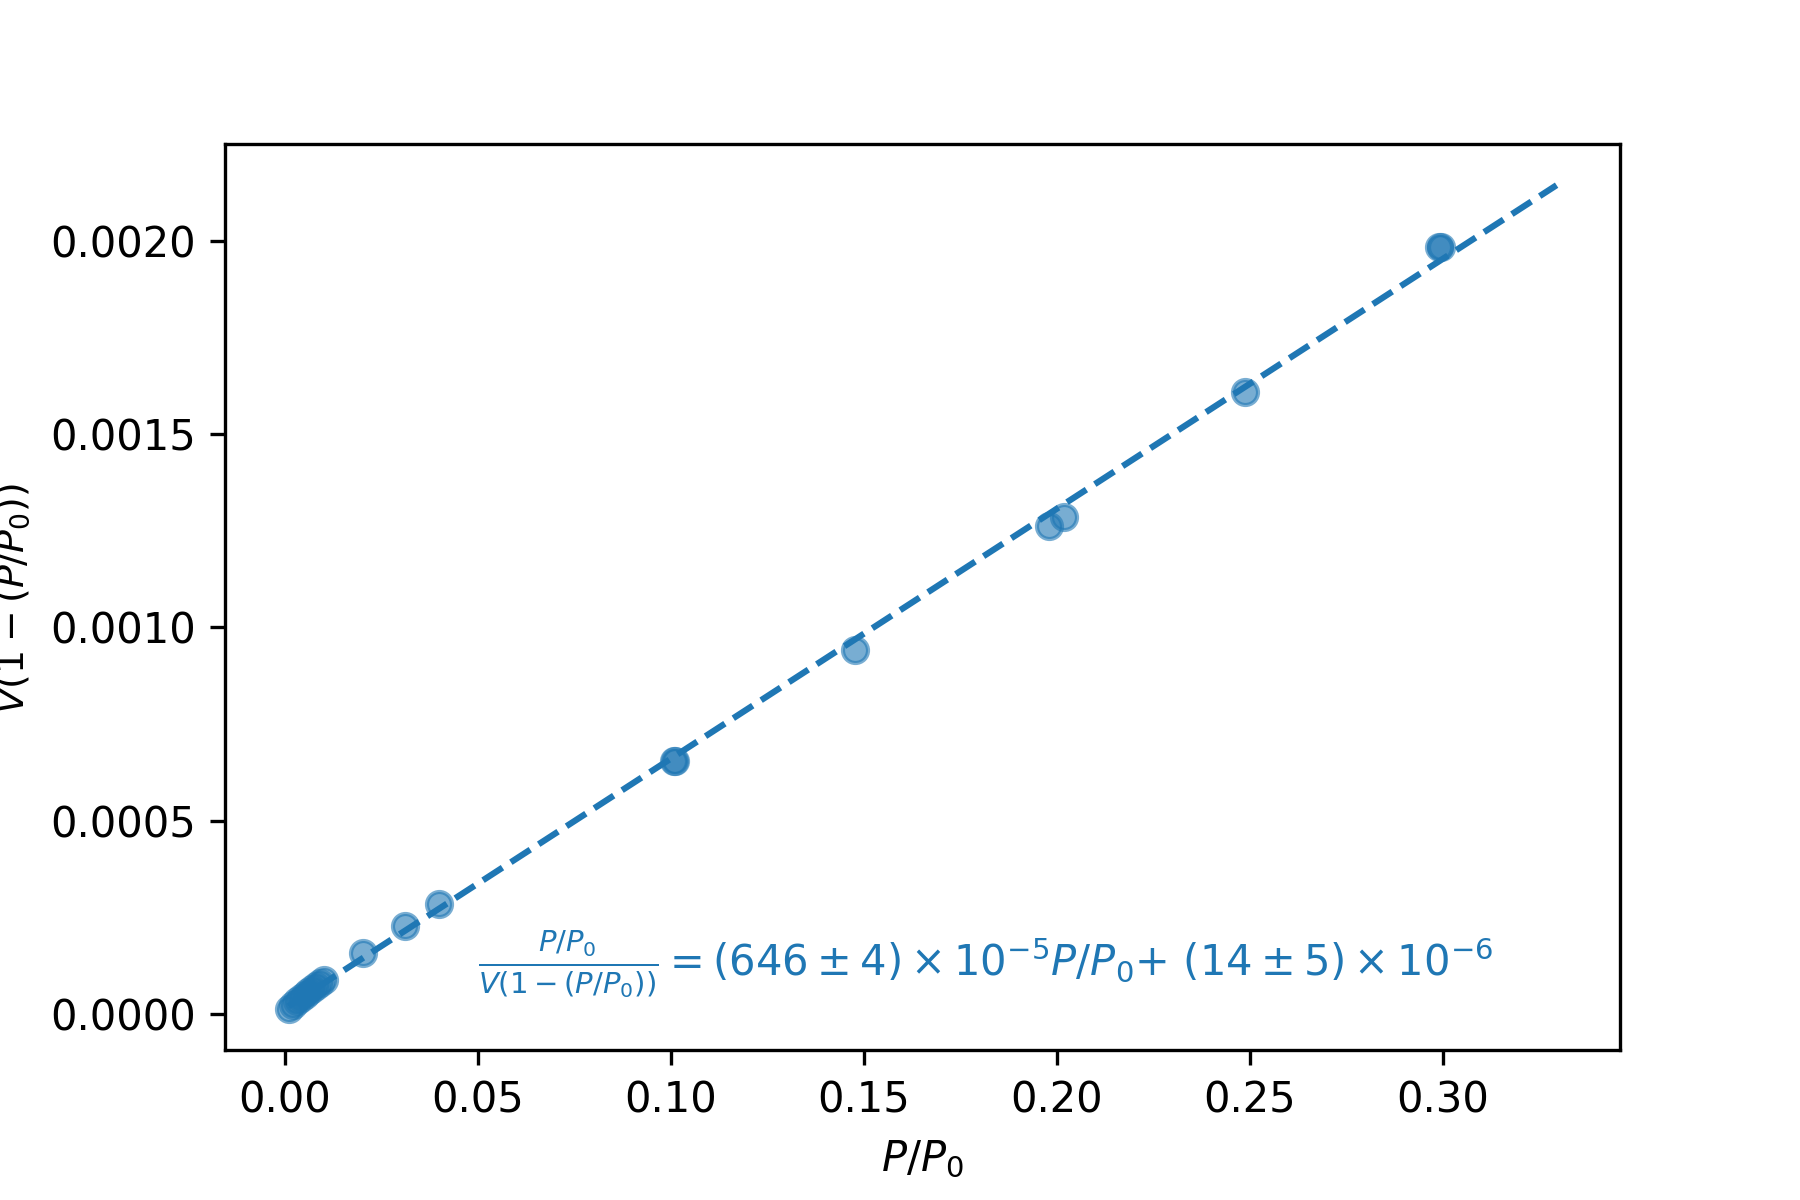
\includegraphics[width=\linewidth]{BET}
		\caption{Diagrama BET, se realiza una regresi\'on lineal sobre el intervalo de presiones relativas de 0.01 a 0,33.}
		\label{fig: bet}
	\end{figure*}
	
	Respecto a las isot\'ermas de adsorci\'on y desorci\'on se observan tres regiones: la adsorci\'on de una monocapa y una multicapa (1), la condensaci\'on capilar (2) y la adsorci\'on en la superficie exterior de las part\'iculas (3), como se observan en la \autoref{fig: isoterma}, los cuales corresponden con una curva caracter\'istica de compuestos mesoporosos, tipo IV \cite{vargas_legnoverde_giraldo_basaldella_moreno-pirajan_2010}.
	
	Como fue mencionado anteriormente, a partir de la isoterma es posible obtener informaci\'on sobre el \'area superficial total del compuesto as\'i como el volumen de la monocapa. Para esto se usa la ecuaci\'on de BET:
	\begin{equation}
		\dfrac{1}{v(P_0/P - 1)} = \dfrac{c-1}{v_mc}\left(\dfrac{P}{P_0}\right) + \dfrac{1}{v_mc}
	\end{equation}
	
	Donde $c$ es la constante BET, la cual cuantifica la magnitud de la interacci\'on adsorbato adsorbente, y $v_m$ corresponde con el volumen de la monocapa. Definiendo $\psi = P/P_0$ como la presi\'on relativa, la ecuaci\'on anterior se reescribe como:
	\begin{equation}
		\dfrac{\psi}{v(1-\psi)} = \left(\dfrac{c-1}{v_mc}\right)\psi + \dfrac{1}{v_mc}
	\end{equation}
	
	Lo anterior implica que al graficar $\psi/(v(1-\psi))$ en funci\'on de la presi\'on relativa, se tendr\'a como pendiente al factor $m = (c-1)/(v_mc)$ y el intercepto estar\'a dado por $b = 1/(v_mc)$. Haciendo expl\'icita la \'ultima expresi\'on para $c$, se obtiene:
	\begin{equation}
		c = \dfrac{1}{v_mb}
	\end{equation}
	
	Sustituyendo en la expresi\'on de la pendiente:
	\begin{equation}
		m = \dfrac{1/(v_mb) - 1}{v_m/(v_mb)} = \dfrac{1-v_mb}{v_m}
	\end{equation}
	
	De donde se obtiene una expresi\'on para el volumen de la monocapa y la constante BET, en funci\'on de los valores de la pendiente y el intercepto de un gr\'afico BET.
	\begin{equation}\label{eq: vmc}
		v_m = \dfrac{1}{m+b}\quad\text{,}\quad
		c = 1 + \dfrac{m}{b}
	\end{equation}
	
	Ahora, la incertidumbre en estos valores ser\'a obtenida usando propagaci\'on de la incertidumbre.
	\begin{equation}
		\delta v_m =
		\sqrt{\left(\dfrac{\partial v_m}{\partial m}\right)^2\delta m^2 + 
		\left(\dfrac{\partial v_m}{\partial b}\right)^2\delta b^2}
	\end{equation}
	
	Donde $\delta m$ y $\delta b$ corresponden con la incertidumbre de la pendiente y el intercepto. En particular se tiene:
	\begin{equation}
		\delta v_m = \dfrac{1}{\left(m + b\right)^2}\sqrt{\delta m^2 + \delta b^2}
	\end{equation}
	\begin{equation}
		\delta c = \dfrac{1}{b}\sqrt{\delta m^2 + \left(\dfrac{m}{b}\right)^2\delta b^2}
	\end{equation}
	
	Con lo anterior se construye la \autoref{fig: bet}, donde la regresi\'on se realiza con los valores en $0.01\leq \psi \leq 0.33$. Con los valores de pendiente obtenidos se obtienen los siguientes valores para la constante BET y el volumen de la monocapa, siguiendo la \autoref{eq: vmc}: $c = 500 \pm 200$, y $v_m = 154 \pm 1$ STP. Con esta informaci\'on se construye la l\'inea segmentada de la \autoref{fig: isoterma}, en donde se observa que esta sigue la tendencia hasta presiones relativas cercanas a 0.4. Lo anterior es de esperarse dado que el modelo de BET es lineal \'unicamente en el rango de los mesoporos \cite{llewellyn2007bet}. Usando el volumen de la monocapa es posible obtener la superficie total, usando la siguiente ecuaci\'on:
	\begin{equation}
		S_{\text{total}} = \dfrac{v_mN\sigma}{V}
	\end{equation}
	
	Donde $N$ es el n\'umero de Avogadro, $\sigma$ la secci\'on eficaz del adsorbato y $V$ el volumen molar del mismo. Dado que el adsorbato es nitr\'ogeno se tiene que $\sigma = 0.162$ nm$^2$ y $V = 22.41$ L/mol \cite{ismail1992cross}. Realizando los cambios de unidades para que todas las longitudes correspondan con metros, se calcula la superficie total en $S_\text{total} = 670 \pm 4$ m$^2$, sin embargo dado que se desconoce la masa de SBA usada, no es posible comparar con la literatura, pues la superficie total es una propiedad extensiva.
	
	\section{Conclusiones}
	Usando la isoterma de adsorci\'on de la SBA-15, fue posible obtener los par\'ametros BET, con su respectiva incertidumbre, a partir de una regresi\'on lineal sobre una gr\'afica BET. El volumen de la monocapa se determin\'o en $v_m = 154\pm 1$ STP y la constante BET $c = 500 \pm 200$. Finalmente, y teniendo en cuenta la secci\'on eficaz del adsorbato nigr\'oteno, se determina el \'area superficial total en $670\pm 4$ m$^2$.
	
	%----------------------------------------------------------------------------------------
	%	REFERENCE LIST
	%----------------------------------------------------------------------------------------
	\phantomsection
	\bibliography{informe}
	\bibliographystyle{achemso}
	
	
\end{document}